\documentclass{article}
\usepackage{amsmath}
\usepackage[utf8]{inputenc} % `utf8` option to match Editor encoding
\usepackage[T1]{fontenc}
\usepackage[ruled,vlined]{algorithm2e}
\usepackage{graphicx}
\graphicspath{ {./} }

\begin{document}
\section{Lista 3, Zadanie 7}
W treści zadanie jest to pominięte, ale przez algorytm sortujący mamy na myśli \textbf{algorytm sortujący za pomocą porównań} (Comparison Model). W pierwszej subsekcji przedstawię prezentacje algorytmu sortujacego za pomocą drzewa decyzyjnego, zaś w drugiej subsekcji przeanalizuję złożoność asymptotyczną dla danych o długościach wymienionych w zadaniu.\\

\subsection{Drzewa decyzyjne}
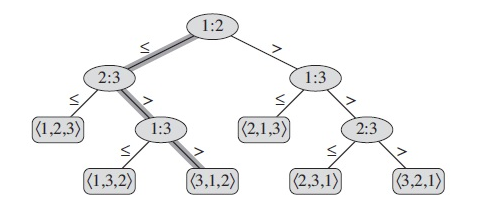
\includegraphics[scale=0.7]{tree}\\
Powyższe drzewo decyzyjne przedstawia algorytm sortujący działający na ciągu 3-elementowym. Węzły wewnętrzne to indeksy elementów które są porównywane, liście natomiast są wszytskimi możliwym permutacjami. Na tej zasadzie właśnie działają algorytmy sortujące. Gdy nie bedziemy myśleć o wartościach elementów, a zamiast tego o ich indeksach, to algorytm sortujący zwraca nam pewną permutację $\pi \in S_n$ indeksów elementów, gdzie $S_n$ to zbiór permutacji o długości $n$.\\
Zauważmy jeszcze, że każde drzewo ma przynajmniej $n!$ liści, jako, że każda permutacja zbioru ${1,2, ... n}$ musi wystąpić przynajmniej raz.\\
Dolne ograniczenie algorytmu stanowi długość najdłuższej ścieżki od korzenia do dowolnego liścia. Stąd ogólnie znana prawda, że dowlony algorytm sortujący za pomocą porównań w przypadku pesymistycznym wymaga $\Omega (nlg(n))$ porównań.\\
Szybki dowód na boku:\\
Oznaczmy: wysokość drzewa - $h$, ilość osiągalnych liści - $l$
\begin{align*}
&n! \leq l \leq 2^h,\\
&lg(n!) \leq h,\\
\\
&lg(n!) = \Omega (nlg(n))
\end{align*}
A więc mamy nasz przypadek pesymistyczny. Co jeżeli zmienimy zakres danych?

\subsection{Mniejszy zakres danych}
Pokażę, że nie istnieje algorytm sortujący CM działający w czasie liniowym dla $m$ różnych danych wejściowych poprzez pokazanie, że wysokość poddrzewa odpowiadajaca tym $m$ permutacją jest asymptotycznie większa niż liniowa.\\
Oznaczmy: \\$m_1 = n!/2, \quad m_2 = n!/n, \quad m_3 = n!/2^{n}$\\ 
$h$ - to dalej wysokość drzewa.\\
$log$ - oznacza logarytm o podstawie 2.\\
\\
Dla $m_1$:
\begin{align*}
m_1 \leq 2^{h} \equiv h &\geq \log m_1 \\&= \log \frac{n!}{2} \\&= \log n! - \log 2 \\&= \log n! - 1 = \Omega(n log (n))
\end{align*}

Dla $m_2$:
\begin{align*}
m_2 \leq 2^{h} \equiv h &\geq \log m_2 \\&= \log \frac{n!}{n} \\&= \log n! - \log n \\&= \log 1 + log 2 + ... + log(n-1) + log(n)  - log(n) \\&\leq log(n) + log(n) + ... + log(n) \\&= n \cdot log(n) = \Omega(n log (n))
\end{align*}

Dla $m_3$:
\begin{align*}
m_3 \leq 2^{h} \equiv h &\geq \log m_3 \\&= \log \frac{n!}{2^{n}} \\&= \log n! - \log 2^{n} \\&= \log n! - n = \Omega(n log n)
\end{align*}

\end{document}